\documentclass[12pt,letterpaper,titlepage]{article}
\usepackage{fancyhdr}
\usepackage{fullpage}
\usepackage{lastpage}
\usepackage{graphicx}
\usepackage{verbatim}

\pdfpagewidth 8.5in
\pdfpageheight 11in
\textwidth 6.5in
\textheight 9in

%\pagestyle{fancyplain}
\pagestyle{fancy}
\lhead[]{Astrometry.net}
\chead[]{}
\rhead[]{Blind Solver: User Notes}
\cfoot[]{\thepage \ of \pageref{LastPage}}
\renewcommand{\headrulewidth}{0.5pt}
\renewcommand{\footrulewidth}{0pt}

\thispagestyle{empty}

\newcommand{\an}{Astrometry.net}
\newcommand{\code}[1]{\texttt{#1}}

\begin{document}
\title{Astrometry.net Blind Solver \\ User Notes}
\author{Dustin Lang}

\maketitle

\newpage

\section{Introduction}

This document is not meant to help you fix problems with building the \an{} code or 
running the basic \code{Makefile}.  These kinds of problems should be reported to the
mailing list.  Rather, this document is meant to help you take the next steps toward
using our code to solve your images.

%We will assume that you have downloaded and built the code and run it on the sample of
%SDSS fields we supplied.

-demo distribution

There are at least three distinct phases of ``the pipeline'' where you might want to
jump in.  For the purposes of this document, we'll start with the Astrometry.net catalog,
which is generated from the raw source catalogs: USNO-B and Tycho-2.  The
process of building the Astrometry.net catalog is deterministic and has no parameters.

\begin{figure}[h!]
\begin{center}
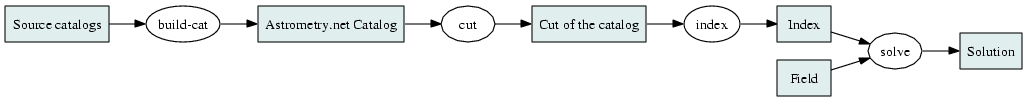
\includegraphics[width=\textwidth]{userdoc-fig-pipeline}
\caption{The blind solver pipeline, writ large.}
\label{fig-pipeline}
\end{center}
\end{figure}

The first major stage of the pipeline is \emph{making a cut}.  This involves selecting a 
spatially-uniform set of stars that is expected to be bright in the band or bands you are
interested in.  The two ``knobs'' of this process are determining which band you want to focus
on, and how spatially uniform you want the cut to be.  There is a trade-off between choosing bright
stars and ensuring that the chosen stars are spatially uniform.

The second major stage of the pipeline is \emph{building an index}.  This involves finding
``quads'': sets of four stars that satisfy particular local geometry constraints.  Again, there
is a tradeoff between building bright quads and ensuring that the quads are uniformly distributed.

The final stage of the pipeline is \emph{solving fields}.  The parameters in this stage tell the
solver where to find its inputs and where to put its output, how hard to work on each field
and how careful to be when deciding on a solution.

We'll go through the stages in reverse order (and ``degree of difficulty'').

\section{Solving}

-background: the solving process: fields (sorted in decreasing brightness),
 quads \& matching, (scale), agreement, verification.

The solver program is called \code{slave} for historical reasons: at one point we envisioned
there being a \code{master} program that would plan how to solve a set of fields, and \code{slave}
workers that would carry out the plan.  In the end, it wasn't really necessary to have a \code{master}.

The \code{slave} program reads its parameters from a text file.  We typically generate a set of
input files by running a script, but if you are solving a few fields, it may just be easier to edit
the input file by hand.

In the demo distribution, the file \code{create-inputs-1} is a shell script that generates
input files for \code{slave}.  In the demo, it only writes one output file, \code{input.000}.
Its contents are shown below.

\begin{figure}[h!]
\begin{center}
\begin{tabular}{|@{\hspace{24pt}}c@{\hspace{24pt}}|}
\hline
\begin{minipage}{0.6\textwidth}
\vspace{10pt}
\begin{verbatim}
index ./sdss-1/sdss-1-02
field sdss-fields/sdssfield01-hp02.xy
fieldid 1
fields 0/2617
solved solved/solved.01
match match/match.00.01
done done/done.00.01
xcol X
ycol Y
sdepth 0
depth 60
cxdx_margin 0.05
parity 0
tol 0.004
fieldunits_lower 0.39
fieldunits_upper 0.41
agreetol 10
verify_dist 4
nagree_toverify 2
overlap_tosolve 0.25
overlap_tokeep 0.25
min_ninfield 50
do_correspond 0
threads 1
quiet
run
\end{verbatim}
%\vspace{10pt}
%\rule{1pt}{5pt}
%\rule{0pt}{0pt}
\end{minipage}%
\\
\rule{0pt}{4pt} \\
\hline
\end{tabular}
\end{center}
\caption{Contents of \code{input.000} file: input file for \code{slave}.}
\label{input000}
\end{figure}

Let us briefly describe the various parameters.

\subsection{Required parameters}
\begin{description}
\item[\code{index <filename>}]: which index should be used.  The
  \code{slave} program will look for the files \code{<filename>.ckdt.fits},
  \code{<filename>.skdt.fits}, and \code{<filename>.quad.fits}.
\item[\code{field <filename>}]: file from which to read fields to solve.
  The program will look for the file \code{<filename>.fits}.
\item[\code{match <filename>}]: where to write the solutions.  This will be
  a FITS file containing a BINTABLE with many columns describing how the
  fields were solved.
\item[\code{depth <integer>}]: how many field objects to look at.
\item[\code{tol <real number>}] (default 0.01): how close in shape do quads
  have to be to be considered ``matching''.
\item[\code{run}]: run the solver with the parameters given.  This can be
  used to include multiple runs in one parameter file.
\end{description}

\subsection{Recommended parameters}
\begin{description}
\item[\code{agreetol <real>}]
\item[\code{verify\_dist <real>}]
\item[\code{nagree\_toverify <int>}]
\item[\code{overlap\_tosolve <real>}]
\item[\code{overlap\_tokeep <real>}]
\item[\code{min\_ninfield <int>}]
\item[\code{fieldunits\_lower <real>}]
\item[\code{fieldunits\_upper <real>}]
\end{description}

\subsection{Optional parameters}
\begin{description}
\item[\code{quiet}]
\item[\code{maxquads <int>}]
\item[\code{cxdx\_margin <real>}]
\item[\code{do\_correspond <0/1>}] (default 1)
\item[\code{xcol <string>}] (default \code{X})
\item[\code{ycol <string>}] (default \code{Y})
\item[\code{fieldid <int>}]
\item[\code{done <filename>}]
\item[\code{solved <filename>}]
\item[\code{solvedserver <hostname:port>}]
\item[\code{firstfield <int>}]
\item[\code{lastfield <int>}]
\item[\code{fields <int>}]
\item[\code{sdepth <int>}] (default 0)
\item[\code{parity <0/1>}] (default 0)
\item[\code{threads <int>}]
\end{description}

\section{Indexing}

\section{Cutting}

\end{document}
